\documentclass[sigconf,screen,nonacm]{acmart}

\AtBeginDocument{%
  \providecommand\BibTeX{{%
    Bib\TeX}}}

\setcopyright{none}

\begin{document}

\title{Multimodal Interaction Project Report: AVSR}
\subtitle{Audio-Visual Speech Recognition}

\author{Diego Mattias Barreto}
\email{barreto.1901707@studenti.uniroma1.it}
\affiliation{%
  \institution{University of Rome La Sapienza}
  \city{Rome}
  \country{Italy}
}

\begin{abstract}
  This report describes the implementation and evaluation of an Audio-Visual Speech Recognition (AVSR) system. The performance of unimodal architectures (Audio-Only and Video-Only) is compared against a multimodal fusion system. The work includes data augmentation techniques, custom training pipelines, and a granular analysis across six signal degradation conditions.
\end{abstract}

\maketitle

\section{Introduction}

Automatic Speech Recognition (ASR) systems perform well in controlled environments, but their performance degrades significantly in real-world scenarios characterized by high levels of background noise, such as the cocktail party effect. Audio-Visual Speech Recognition (AVSR) seeks to overcome this limitation by leveraging the visual modality --- specifically the speaker's lip movements --- as an additional and orthogonal source of information. Since visual features are invariant to acoustic noise, multimodal fusion can in theory compensate for audio signal degradation when it is heavily corrupted.

Despite the theoretical advantages of AVSR, building robust multimodal systems involves several practical challenges. First, naive padding strategies can introduce a duration bias (\textit{Padding Leakage}), allowing recurrent neural networks to bypass feature extraction by simply counting padding frames. Second, improper dataset splitting can cause data leakage, where the model memorizes the acoustic signature of a specific recording instead of generalizing. Finally, multimodal architectures may be subject to \textit{Negative Transfer}: a degraded input in one modality can corrupt the correct predictions of the other, leading to accuracy lower than the best unimodal baseline.

This project implements an AVSR pipeline addressing these issues. A custom dataset of 10 Italian spoken commands is built, from which MFCC features and MediaPipe facial landmarks are extracted. Static geometric features are enriched with their first and second temporal derivatives ($\Delta$ and $\Delta\Delta$). A ``Continuous Noise Canvas'' technique is introduced to eliminate padding bias, and a Stratified Group K-Fold strategy is adopted to guarantee the absence of data leakage.

The main contributions of this work are:
\begin{itemize}
  \item \textbf{Multimodal architecture:} An Early Fusion architecture is designed and trained, combining an Audio-LSTM and a Video-Bidirectional LSTM, enhanced with Masking and Batch Normalization.
  \item \textbf{Elimination of experimental biases:} Padding bias and data leakage are systematically identified and resolved, ensuring that the models learn genuine phonetic and visual patterns.
  \item \textbf{Ablation matrix:} A 6-condition evaluation matrix (Clean, Audio Light/Heavy, Video Light/Heavy, A+V Light) is constructed to empirically verify modality orthogonality, multimodal synergy, and the negative transfer phenomenon.
\end{itemize}

The rest of the report is organized as follows: Section 2 describes the dataset and feature extraction; Section 3 discusses the experimental methodology; Section 4 presents the model architectures; Section 5 describes training details; Section 6 analyzes the results; Section 7 concludes the work.

\section{Related Work}

The field of AVSR has a long history, starting from the pioneering work of McGurk and McDonald \cite{mcgurk1976}, who demonstrated the influence of the visual signal on speech perception (the McGurk effect). Since then, many systems have sought to exploit this complementarity to build more robust recognizers.

\textbf{Classical approaches.} Early AVSR systems relied on Hidden Markov Models (HMM) with manually crafted visual features (mouth shape, lip distance). These systems showed improvements over acoustic-only models under noisy conditions, but were limited by the quality of the visual features and the rigidity of the generative model.

\textbf{Deep Learning approaches.} With the advent of deep neural networks, more flexible approaches emerged. Convolutional networks (CNN) have been used to automatically extract visual features from mouth pixels, while LSTMs replaced HMMs for temporal modeling. Works such as LipNet \cite{assael2016lipnet} demonstrated that it is possible to train an end-to-end lip-reading system on continuous sequences, achieving human-comparable performance on certain benchmarks.

\textbf{Multimodal fusion.} Fusion strategies can be classified into three categories: Early Fusion (feature-level fusion, as in this work), Late Fusion (fusion of unimodal model predictions), and Hybrid Fusion. The optimal choice depends on the amount of available data and the correlation between modalities. More recent approaches based on Cross-Modal Attention mechanisms and Transformer architectures enable adaptive fusion that dynamically weights modalities according to their contextual reliability.

This work is distinguished from prior work by its focus on rigorously preventing experimental biases (padding leakage and data leakage), an aspect often overlooked in the literature when working with small-scale datasets.

\section{Dataset and Preprocessing}

To train and evaluate the multimodal architecture, a custom Audio-Visual dataset was built. The preprocessing pipeline was designed to extract robust representations from both modalities while preserving their temporal synchronization.

\subsection{Custom Multimodal Dataset}
The dataset comprises synchronized audio and video recordings of ten Italian commands: \textit{avvia, stop, sopra, sotto, sinistra, destra, apri, chiudi, si, no}. These commands were chosen for their practical applicability in human-computer interaction and for the diversity of their phonetic and visemic profiles. The raw data consists of WAV audio files and corresponding MP4 video files. To ensure realistic variability, samples exhibit natural variations in speech duration, pitch, and head movements.

\subsection{Audio Feature Extraction}
Acoustic features were extracted using the \textit{librosa} library. Raw audio signals were resampled to 16 kHz to ensure uniformity. 13 Mel-Frequency Cepstral Coefficients (MFCCs) were computed for each audio frame. MFCCs were chosen because they provide a compact and effective representation of the short-term power spectrum of the vocal tract, isolating speech formants from raw acoustic energy.

Raw spectrograms were considered but discarded because they encode absolute energy levels, making the model sensitive to recording volume rather than phonetic content. MFCCs decorrelate the spectral envelope via the DCT, providing a speaker-independent representation. Thirteen coefficients were chosen as a standard trade-off: fewer coefficients lose formant detail, more add noise-heavy high-frequency information with diminishing phonetic value.

The resulting feature vectors were temporally aligned to a fixed maximum length of 30 frames, yielding a target shape of $(30, 13)$ per sample.

The maximum length of 30 frames was empirically set to cover the 95th percentile of sample durations in the dataset, minimizing padding overhead while avoiding truncation of legitimate speech content.

\subsection{Video Feature Extraction and Kinematics}
Extracting meaningful visual features directly from raw video pixels is computationally expensive and sensitive to background and lighting variations. To isolate the region of interest, the Google MediaPipe Face Mesh framework was used to detect and track specific 3D facial landmarks localized around the speaker's mouth.

Initially, three static geometric measurements were computed per frame: inner lip aperture, outer lip aperture, and horizontal lip width. Preliminary tests revealed, however, that static geometric configurations are insufficient to capture the fluid phonetic patterns of human speech: they yield low feature entropy and cause early gradient stagnation in recurrent networks.

To address this limitation, the temporal dynamics of the lips were explicitly modeled by computing the first and second spatial derivatives (velocities and accelerations, $\Delta$ and $\Delta\Delta$) of the static measurements along the time axis. This kinematic feature engineering expanded the visual feature space from 3 to 9 continuous values per frame, transforming the input from static shapes to dynamic physical trajectories. The final visual input tensor per sample has shape $(30, 9)$.

End-to-end pixel-based approaches (e.g., CNN on mouth crops) were considered but rejected due to dataset size: with fewer than 300 training samples, a CNN would overfit to background and lighting conditions before learning visemic patterns. The geometric keypoint approach reduces the visual input to 3 physically meaningful coordinates, and the $\Delta/\Delta\Delta$ derivatives were added after preliminary tests showed static geometry alone caused gradient stagnation --- the network had no signal to distinguish, say, \textit{apri} from \textit{avvia} based on lip shape alone.

\subsection{Feature Normalization}
Neural networks are highly sensitive to unscaled inputs and artificial numerical discontinuities. To ensure stable gradient propagation through the LSTM layers, video feature matrices are subjected to explicit Z-score normalization (zero mean, unit variance) as a preprocessing step before training, computed on the training set and applied to validation and test sets. Audio features are instead normalized internally: the first layer of both the audio branch and the fusion model is a \textit{Batch Normalization} layer, which standardizes the MFCC distribution online during training. This normalization is essential to allow the Masking layers to correctly ignore temporal padding and to prevent the vanishing gradient phenomenon observed in preliminary tests.

\section{Experimental Methodology}

One of the main challenges in training Deep Learning models for time-series classification is preventing the network from learning artificial heuristics instead of the intended phenomena. This section describes the methodological choices adopted.

\subsection{Preventing Data Leakage: Stratified Group K-Fold}
\label{sec:splitting}
Standard randomized splitting techniques (e.g., \textit{train-test split}) present a critical problem when applied to augmented datasets. In preliminary tests, standard splitting caused augmented variants of the same physical recording (e.g., the ``clean'' version and its ``heavy noise'' counterpart) to appear in both the training and validation sets. As a result, the network memorized the speaker's specific acoustic signature, achieving an artificially high accuracy of 100\% even under severe -15dB noise.

\begin{sloppypar}
  To definitively eliminate data leakage, the splitting pipeline adopts a two-stage
  \textit{Stratified Group K-Fold} strategy. First, a \texttt{Stratified}\allowbreak\texttt{GroupKFold}
  with $n\_splits=7$ is used to carve out a fixed, held-out Test set. The remaining
  data is then split into training and validation sets using a second
  \texttt{Stratified}\allowbreak\texttt{GroupKFold} with $n\_splits=5$. In both stages only the first
  fold of the iterator is used, yielding a single fixed train/val/test partition
  rather than a full cross-validation loop. The base filename of each raw recording
  is designated as the distinct ``group'' identifier, guaranteeing that all augmented
  variants of a recording fall entirely within the same partition. The stratification
  component enforces class balance across all three splits.
\end{sloppypar}

\subsection{Mitigating Padding Bias: Continuous Noise Canvas}
Sequence models such as LSTMs require fixed-length input tensors, making it necessary to pad variable-length samples. The initial approach used standard zero-padding to reach the target length of 30 frames. Diagnostic audits revealed, however, a profound ``Padding Leakage'' (duration bias): the LSTM was not extracting phonetic features from the augmented audio but was instead counting the number of zero-valued frames to infer the original duration of the spoken word.

To eliminate this heuristic shortcut, zero-padding was abandoned in favor of the ``Continuous Noise Canvas'' technique. Instead of appending zeros to the truncated audio signal, a continuous canvas of environmental noise matching the target maximum length is generated. The isolated speech waveform is then superimposed (mixed) onto this canvas at a randomized temporal offset. By ensuring that every matrix element contains non-zero acoustic data, the duration bias is completely eliminated.

Keras's \texttt{Masking} layer was the first mitigation strategy considered: it instructs the LSTM to skip timesteps where all features equal exactly zero. However, diagnostic experiments showed the LSTM had already learned to count non-masked frames before the Masking fix was applied, and validation accuracy remained suspiciously high for short commands. The Continuous Noise Canvas eliminates the shortcut at the source --- by ensuring every frame contains non-zero acoustic data, duration becomes informationally invisible to the network.

\subsection{Multimodal Augmentation Strategy}
To empirically test the orthogonal independence and synergistic gating capabilities of the fusion model, a set of targeted unimodal degradations was constructed.

For the acoustic modality, non-stationary \textit{Babble Noise} (cocktail party effect) was used, as it occupies the same frequency bands as human speech. The noise was applied at two distinct SNR levels: +5dB (Light Augmentation) and -15dB (Heavy Augmentation).

For the visual modality, spatial \textit{Jitter} (rapid frame-by-frame coordinate perturbation) was introduced to simulate camera instability (Light Augmentation) and a static \textit{Tilt} to simulate off-axis framing (Heavy Augmentation).

These isolated degradation strategies formed the basis for the 6-condition \textit{Ablation Matrix} (Clean, Audio Light, Audio Heavy, Video Light, Video Heavy, Audio+Video Light).

White Gaussian noise was initially used for acoustic degradation but rejected because it is spectrally flat and easy to filter: the LSTM quickly learned to discount it. Babble noise (overlapping human voices) was chosen because it occupies the same frequency bands as the target speech, making spectral filtering impossible. For the visual modality, Gaussian blur was considered but found to leave landmark topology intact; Jitter was chosen instead because it directly destroys the $\Delta/\Delta\Delta$ derivatives, which are the model's primary visual signal.

\section{Model Architectures}

To compare the benefits of multimodal integration, three distinct neural network architectures were designed: an Audio-Only baseline, a Video-Only baseline, and an Early Fusion multimodal network. All models were implemented with the Keras/TensorFlow framework and optimized for the classification of temporal sequences into 10 command classes.

\subsection{Audio-Only Baseline}

\begin{figure}[ht]
  \centering
  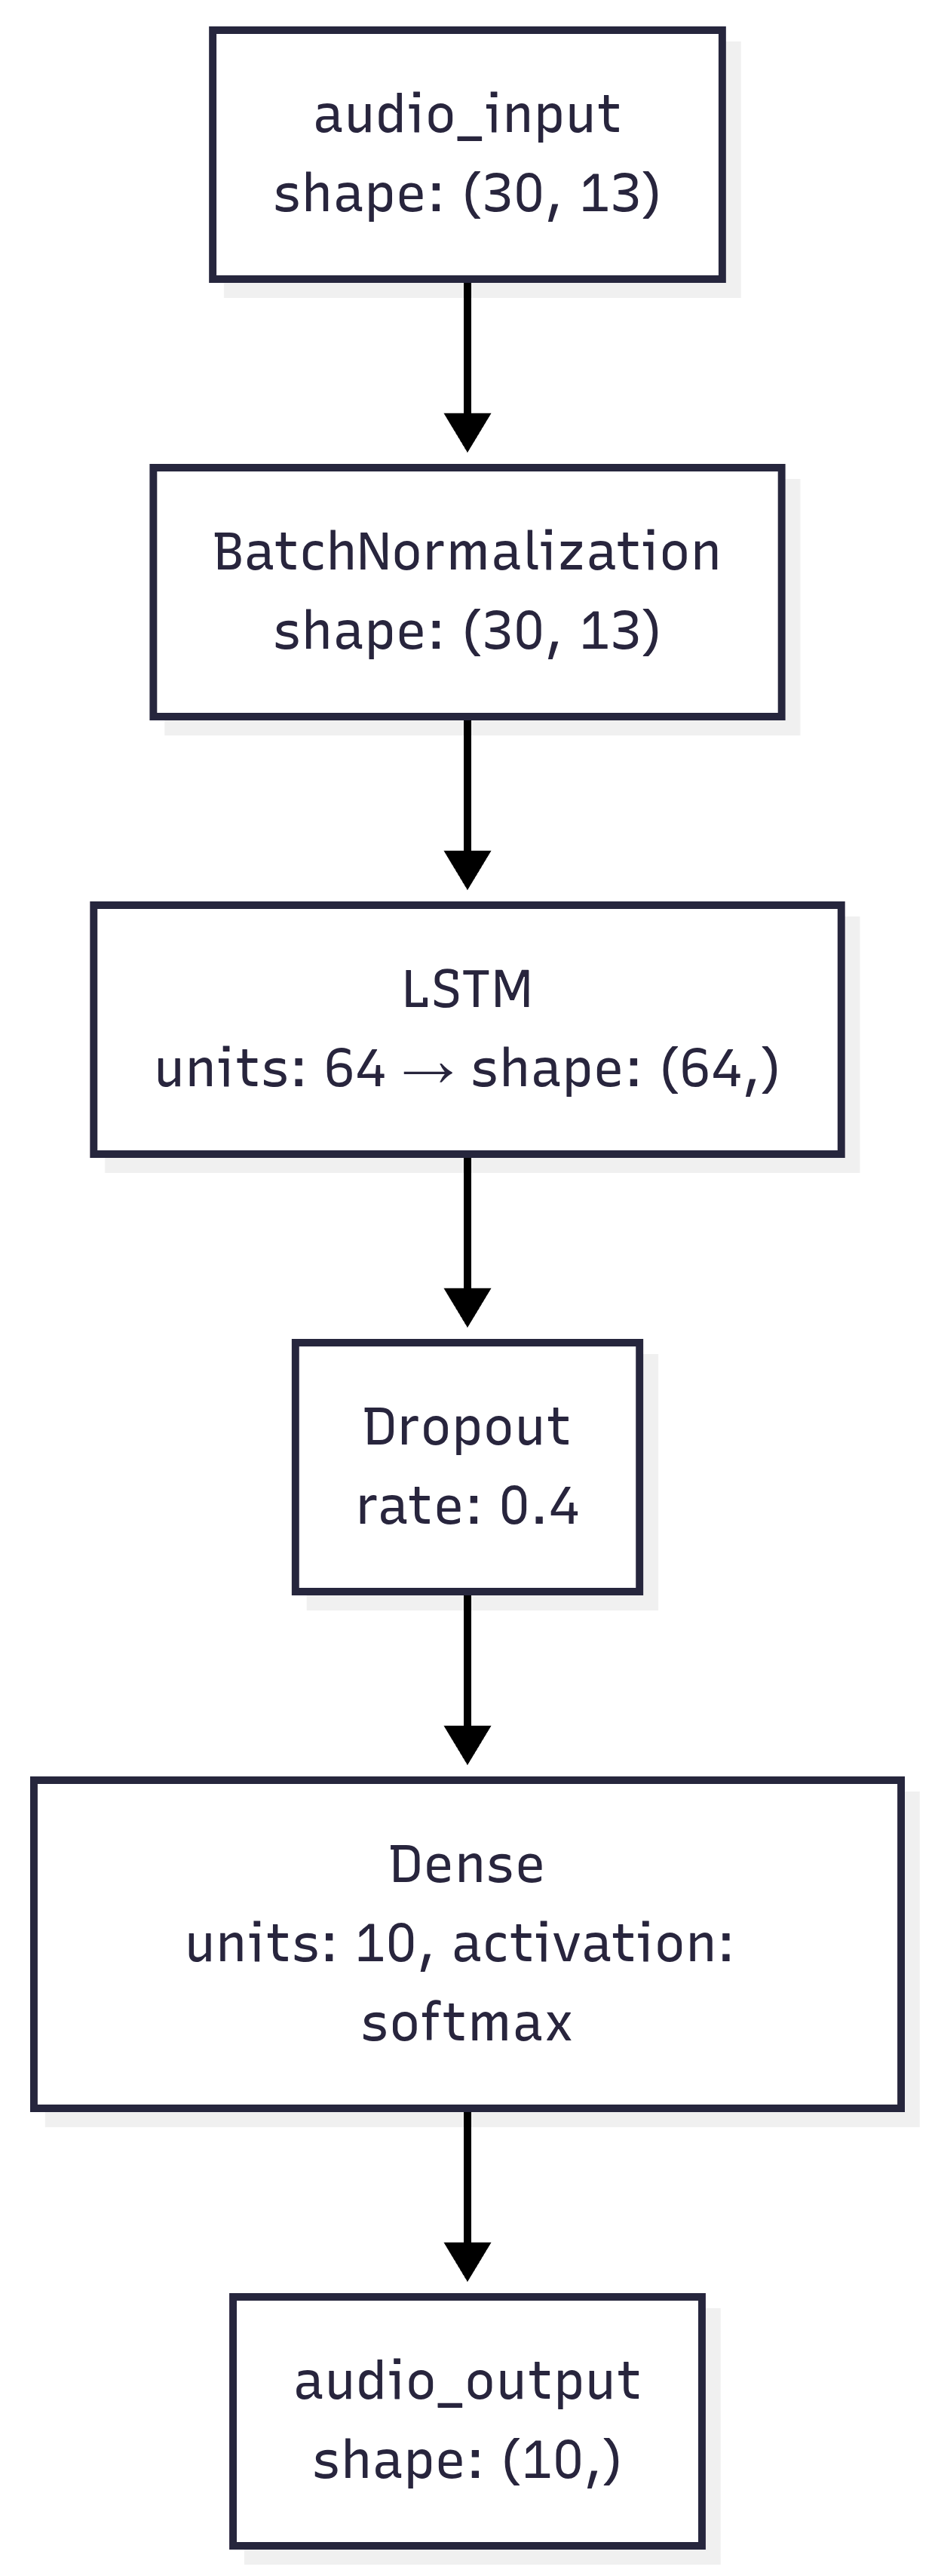
\includegraphics[width=0.55\columnwidth]{assets/Audio_model.png}
  \caption{Architecture of the Audio-Only LSTM model.}
  \label{fig:arch_audio}
\end{figure}

The acoustic baseline is a unimodal recurrent neural network designed to process MFCC sequences. The input tensor, shaped $(T, F_A)$ with $T=30$ temporal frames and $F_A=13$ acoustic features, is first processed by a \textit{Batch Normalization} layer, which standardizes the distribution of acoustic formants and accelerates optimizer convergence.

The normalized sequence is then passed to a unidirectional LSTM layer with 64 hidden units, which captures the temporal dependencies of the speech signal. To mitigate overfitting, a Dropout layer with rate 0.4 precedes the final Dense layer with Softmax activation, which produces the probability distribution over the 10 target classes.

GRU was considered as a lighter alternative to LSTM, offering fewer parameters with comparable performance on short sequences. Preliminary experiments showed marginal accuracy differences between the two, so LSTM was retained for its wider adoption in the AVSR literature, making results more directly comparable. Transformer-based encoders were excluded due to dataset size: self-attention requires significantly more data to learn meaningful positional relationships and tends to overfit on small corpora like ours.

\subsection{Video-Only Baseline}

\begin{figure}[ht]
  \centering
  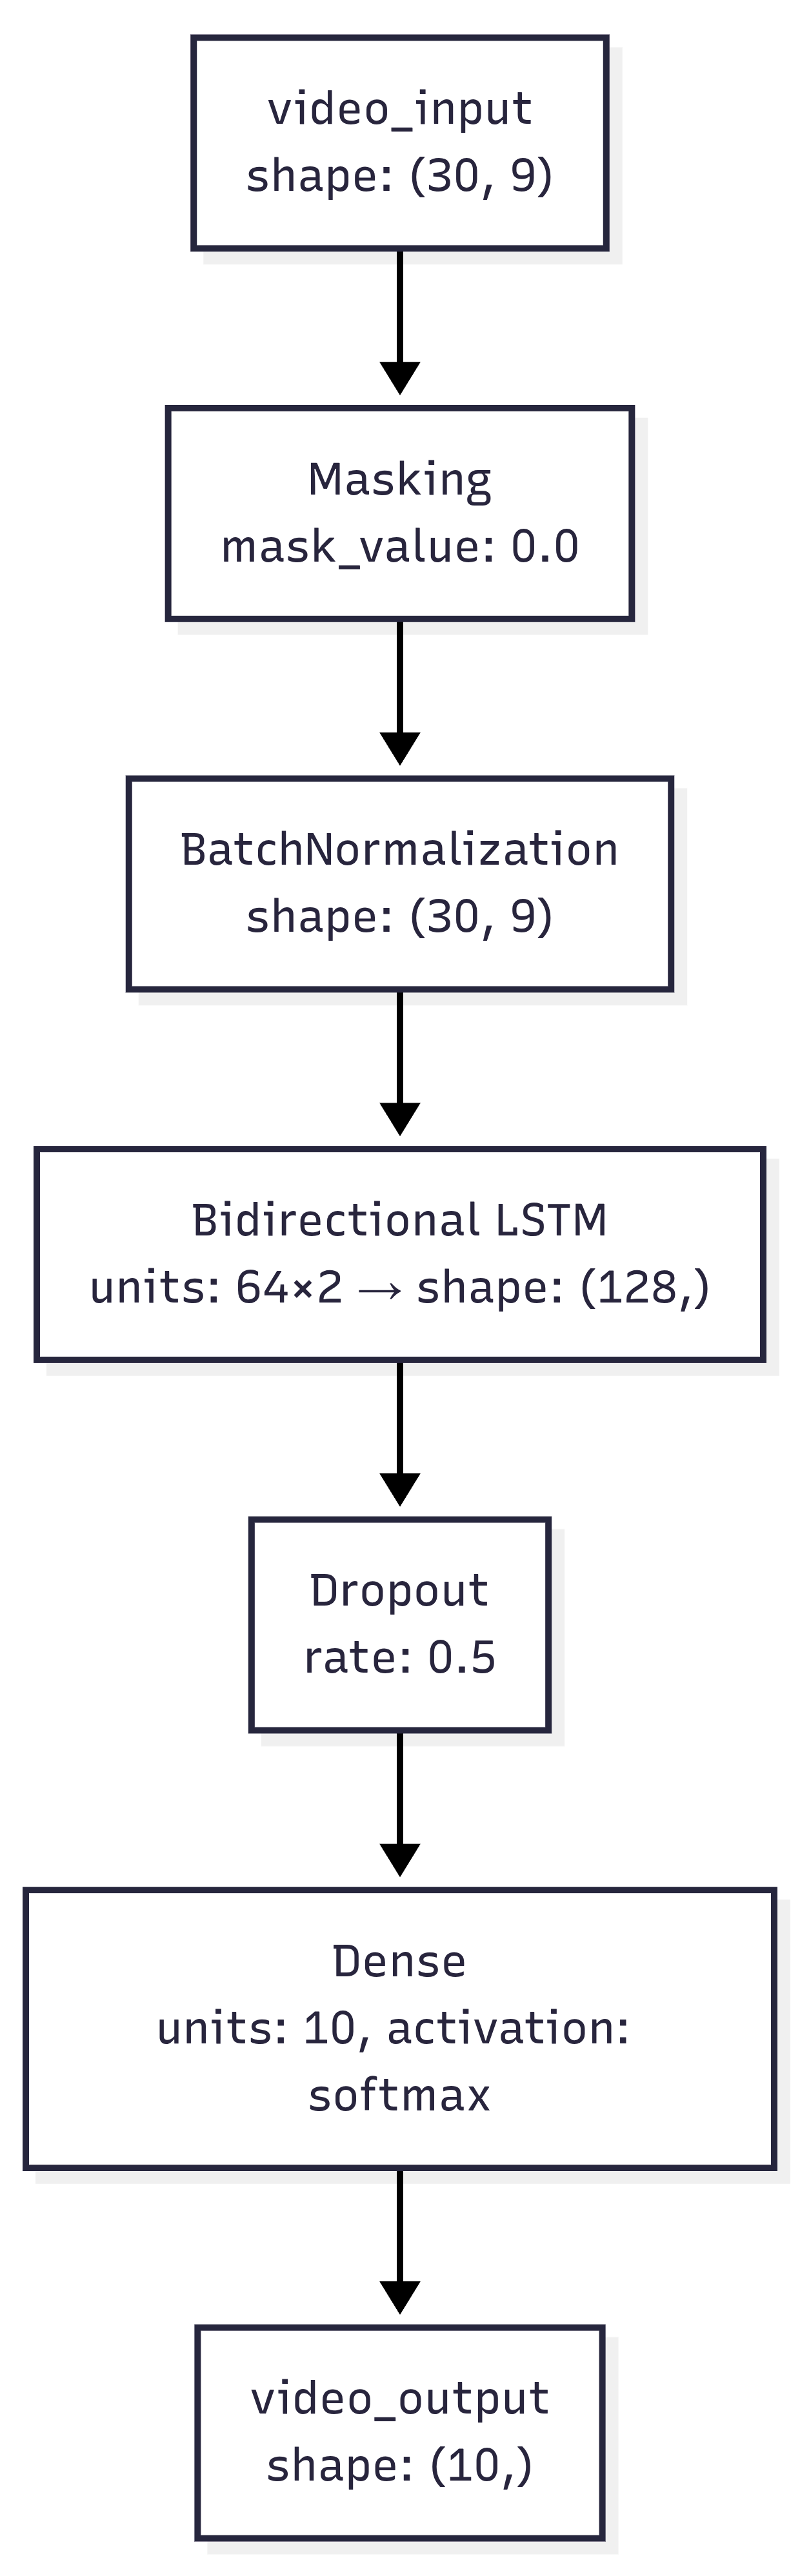
\includegraphics[width=0.55\columnwidth]{assets/video_model.png}
  \caption{Architecture of the Video-Only BiLSTM model.}
  \label{fig:arch_video}
\end{figure}

The visual baseline is designed to interpret the spatiotemporal kinematics of the speaker's lips. The input tensor has shape $(T, F_V)$ with $F_V=9$ kinematic features.

A critical component of this architecture is the initial \textit{Masking} layer (configured with \texttt{mask\_value=0.0}). Without masking, the LSTM would interpret the artificial transitions from legitimate geometric coordinates to exact zeros as extreme, instantaneous physical movements, causing gradient collapse.

After Batch Normalization, the data is processed by a \textit{Bidirectional LSTM} layer with 64 units. Unlike the acoustic model, lip-reading greatly benefits from bidirectional context: understanding a current viseme often requires knowledge of how the lips will close or open in the immediate future. The BiLSTM concatenates the forward and backward hidden states, passing them through a heavy Dropout (0.5) to the Softmax classification head.

The asymmetry between a unidirectional LSTM (audio) and a BiLSTM (video) reflects a fundamental difference in the two modalities' temporal structure. Speech formants unfold causally: the acoustic realization of a phoneme depends on what came before, not what comes after. Lip movements, by contrast, exhibit coarticulation --- the mouth begins preparing the shape for an upcoming phoneme before the current one is complete. A BiLSTM's backward pass captures this anticipatory motion, which a unidirectional model cannot see.

\subsection{Multimodal Early Fusion Model}

\begin{figure*}[!ht]
  \centering
  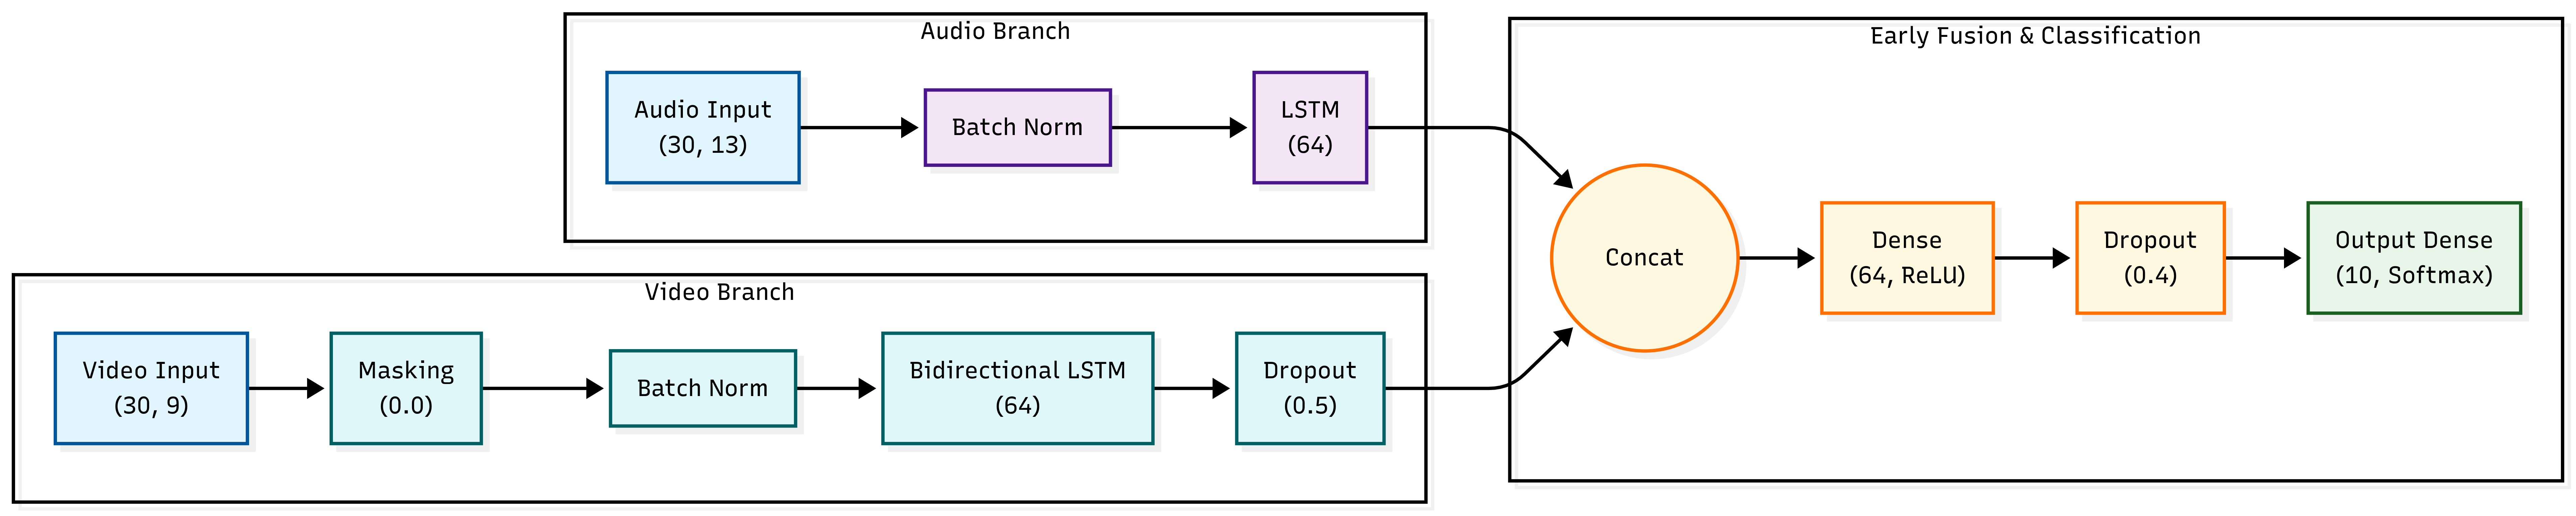
\includegraphics[width=\textwidth]{assets/Audio-Video Fusion Model.png}
  \caption{Architecture of the proposed Audio-Visual Early Fusion model.}
  \label{fig:fusion_model}
\end{figure*}

The proposed AVSR system adopts a feature-level Early Fusion strategy to integrate the acoustic and visual modalities. The network consists of two parallel feature-extraction branches:
\begin{itemize}
  \item \textbf{Acoustic Branch:} Processes MFCCs through a Batch Normalization layer and a 64-unit LSTM.
  \item \textbf{Visual Branch:} Processes kinematic lip features through a Masking layer, Batch Normalization, and a 64-unit Bidirectional LSTM, followed by a 0.5 Dropout.
\end{itemize}
Instead of generating independent predictions, the final hidden states from both branches are merged via a \textit{Concatenate} layer. The combined multimodal feature vector is then projected into a shared representational space via a Dense layer with 64 units and ReLU activation. This cross-modal projection allows the network to learn non-linear correlations between auditory formants and visual kinematics (e.g., associating the acoustic silence of a consonant with the visual closure of the lips). A final Dropout layer (0.4) precedes the 10-class Softmax output layer.

Late Fusion --- training two independent classifiers and averaging their softmax outputs --- was considered for its simplicity. It was rejected because it forces each modality to independently reach a classification decision before fusion, losing any cross-modal correlations at the feature level. Hybrid Fusion was deemed premature given the dataset scale. Early Fusion was chosen as the best trade-off: by concatenating the LSTM hidden states before classification, the shared Dense layer can learn non-linear correlations between acoustic formants and visual kinematics --- associations that neither branch could discover alone.

\section{Training Details}

All three models were trained with the same configuration to ensure comparability of results. The optimizer used is Adam with an initial learning rate of $1 \times 10^{-3}$. The loss function adopted is \textit{Categorical Crossentropy}. Training was conducted for a maximum of 100 epochs with a batch size of 32, using an Early Stopping callback (patience = 15) monitoring validation loss to prevent overfitting.

SGD with momentum was considered as an alternative optimizer, but Adam was preferred for its adaptive per-parameter learning rates, which prove beneficial when gradients flow through two branches with different input scales (MFCCs vs.\ kinematic features). The initial learning rate of $1 \times 10^{-3}$ is Adam's standard default and was not tuned further, as preliminary sweeps showed no significant sensitivity in this range. Early Stopping with \texttt{patience=15} was set deliberately high to avoid terminating runs during the noisy middle epochs typical of LSTM training on small datasets; a patience of 5 caused premature stopping before the validation loss plateaued.

\subsection{Dataset Split}

The dataset is split using the two-stage \textit{Stratified Group K-Fold} strategy
described in Section~\ref{sec:splitting}: a fixed test set is carved out first
($n\_splits=7$), and the remainder is divided into training and validation sets
($n\_splits=5$). A single fixed partition is used throughout training and
evaluation; no fold-averaging is performed. Group-based splitting guarantees that
all augmented variants of the same recording stay within the same partition,
preventing any form of data leakage.

A simple random train-test split was the first approach attempted. It produced 100\% accuracy under -15dB noise --- a clear red flag. Investigation revealed that augmented variants of the same recording were appearing in both training and test sets, allowing the model to memorize the speaker's acoustic fingerprint. \texttt{GroupKFold} was introduced to enforce the constraint that all augmented copies of a recording stay in the same partition; the stratification component was added on top to maintain class balance, which would otherwise skew toward commands with more recordings.

\subsection{Parameter Summary}

Table~\ref{tab:params} summarizes the main parameters of the three architectures.

\begin{table}[ht]
  \caption{Summary of the main parameters of the three models.}
  \label{tab:params}
  \centering
  \begin{tabular}{l c c c}
    \toprule
    \textbf{Parameter}  & \textbf{Audio} & \textbf{Video} & \textbf{Fusion} \\
    \midrule
    LSTM Units          & 64             & 64 (Bi)        & 64 + 64 (Bi)    \\
    Input features      & 13 (MFCC)      & 9 (kin.)       & 13 + 9          \\
    Dropout             & 0.4            & 0.5            & 0.4 / 0.5       \\
    Shared Dense        & ---            & ---            & 64 (ReLU)       \\
    Output classes      & 10             & 10             & 10              \\
    Batch Normalization & Yes            & Yes            & Yes             \\
    Masking             & No             & Yes            & Yes             \\
    \bottomrule
  \end{tabular}
\end{table}

\section{Experiments and Results}

To empirically validate the proposed architecture and assess its robustness under varying environmental conditions, the models were evaluated on a 6-condition Ablation Matrix built from the Test set.

\subsection{Ablation Matrix Setup}
The Test set was augmented to create six strictly isolated conditions for each original sample:
\begin{enumerate}
  \item \textbf{Clean}: Unaltered audio and video.
  \item \textbf{Audio Light}: Babble Noise at 5dB SNR.
  \item \textbf{Audio Heavy}: Babble Noise at -15dB SNR.
  \item \textbf{Video Light}: High-frequency spatial Jitter.
  \item \textbf{Video Heavy}: Static spatial Tilt.
  \item \textbf{A+V Light}: Simultaneous 5dB SNR noise and spatial Jitter.
\end{enumerate}

The six conditions were not chosen arbitrarily: each is designed to isolate a specific hypothesis. Clean establishes the performance ceiling. Audio Light/Heavy tests graceful degradation of the acoustic branch in isolation. Video Light/Heavy does the same for the visual branch. A+V Light is the critical stress test for modality interference --- both branches receive degraded input simultaneously, which is the scenario where Early Fusion is most likely to fail. This structure allows each cell in Table~\ref{tab:results} to answer a specific scientific question rather than reporting aggregate accuracy on a heterogeneous test set.

Table~\ref{tab:results} reports the granular accuracy scores across all conditions.

\begin{table*}[h]
  \caption{Granular evaluation results across the different degradation conditions.}
  \label{tab:results}
  \centering
  \begin{tabular}{l c c c c c c c}
    \toprule
    \textbf{Model}        & \textbf{Overall} & \textbf{Clean}    & \textbf{Aud. Light} & \textbf{Aud. Heavy} & \textbf{Vid. Light} & \textbf{Vid. Heavy} & \textbf{A+V Light} \\
    \midrule
    Audio-Only LSTM       & 90.23\%          & 100.00\%          & 100.00\%            & 44.83\%             & 100.00\%            & 100.00\%            & 96.55\%            \\
    Video-Only BiLSTM     & 77.01\%          & 96.55\%           & 96.55\%             & 96.55\%             & 41.38\%             & 96.55\%             & 34.48\%            \\
    \textbf{Early Fusion} & \textbf{96.55\%} & \textbf{100.00\%} & \textbf{100.00\%}   & \textbf{86.21\%}    & \textbf{96.55\%}    & \textbf{100.00\%}   & \textbf{96.55\%}   \\
    \bottomrule
  \end{tabular}
\end{table*}

\subsection{Learning Curves}

The learning curves of the three models are shown in the figures below and illustrate the trend of accuracy and loss on the training and validation sets during training.

\begin{figure*}[h]
  \centering
  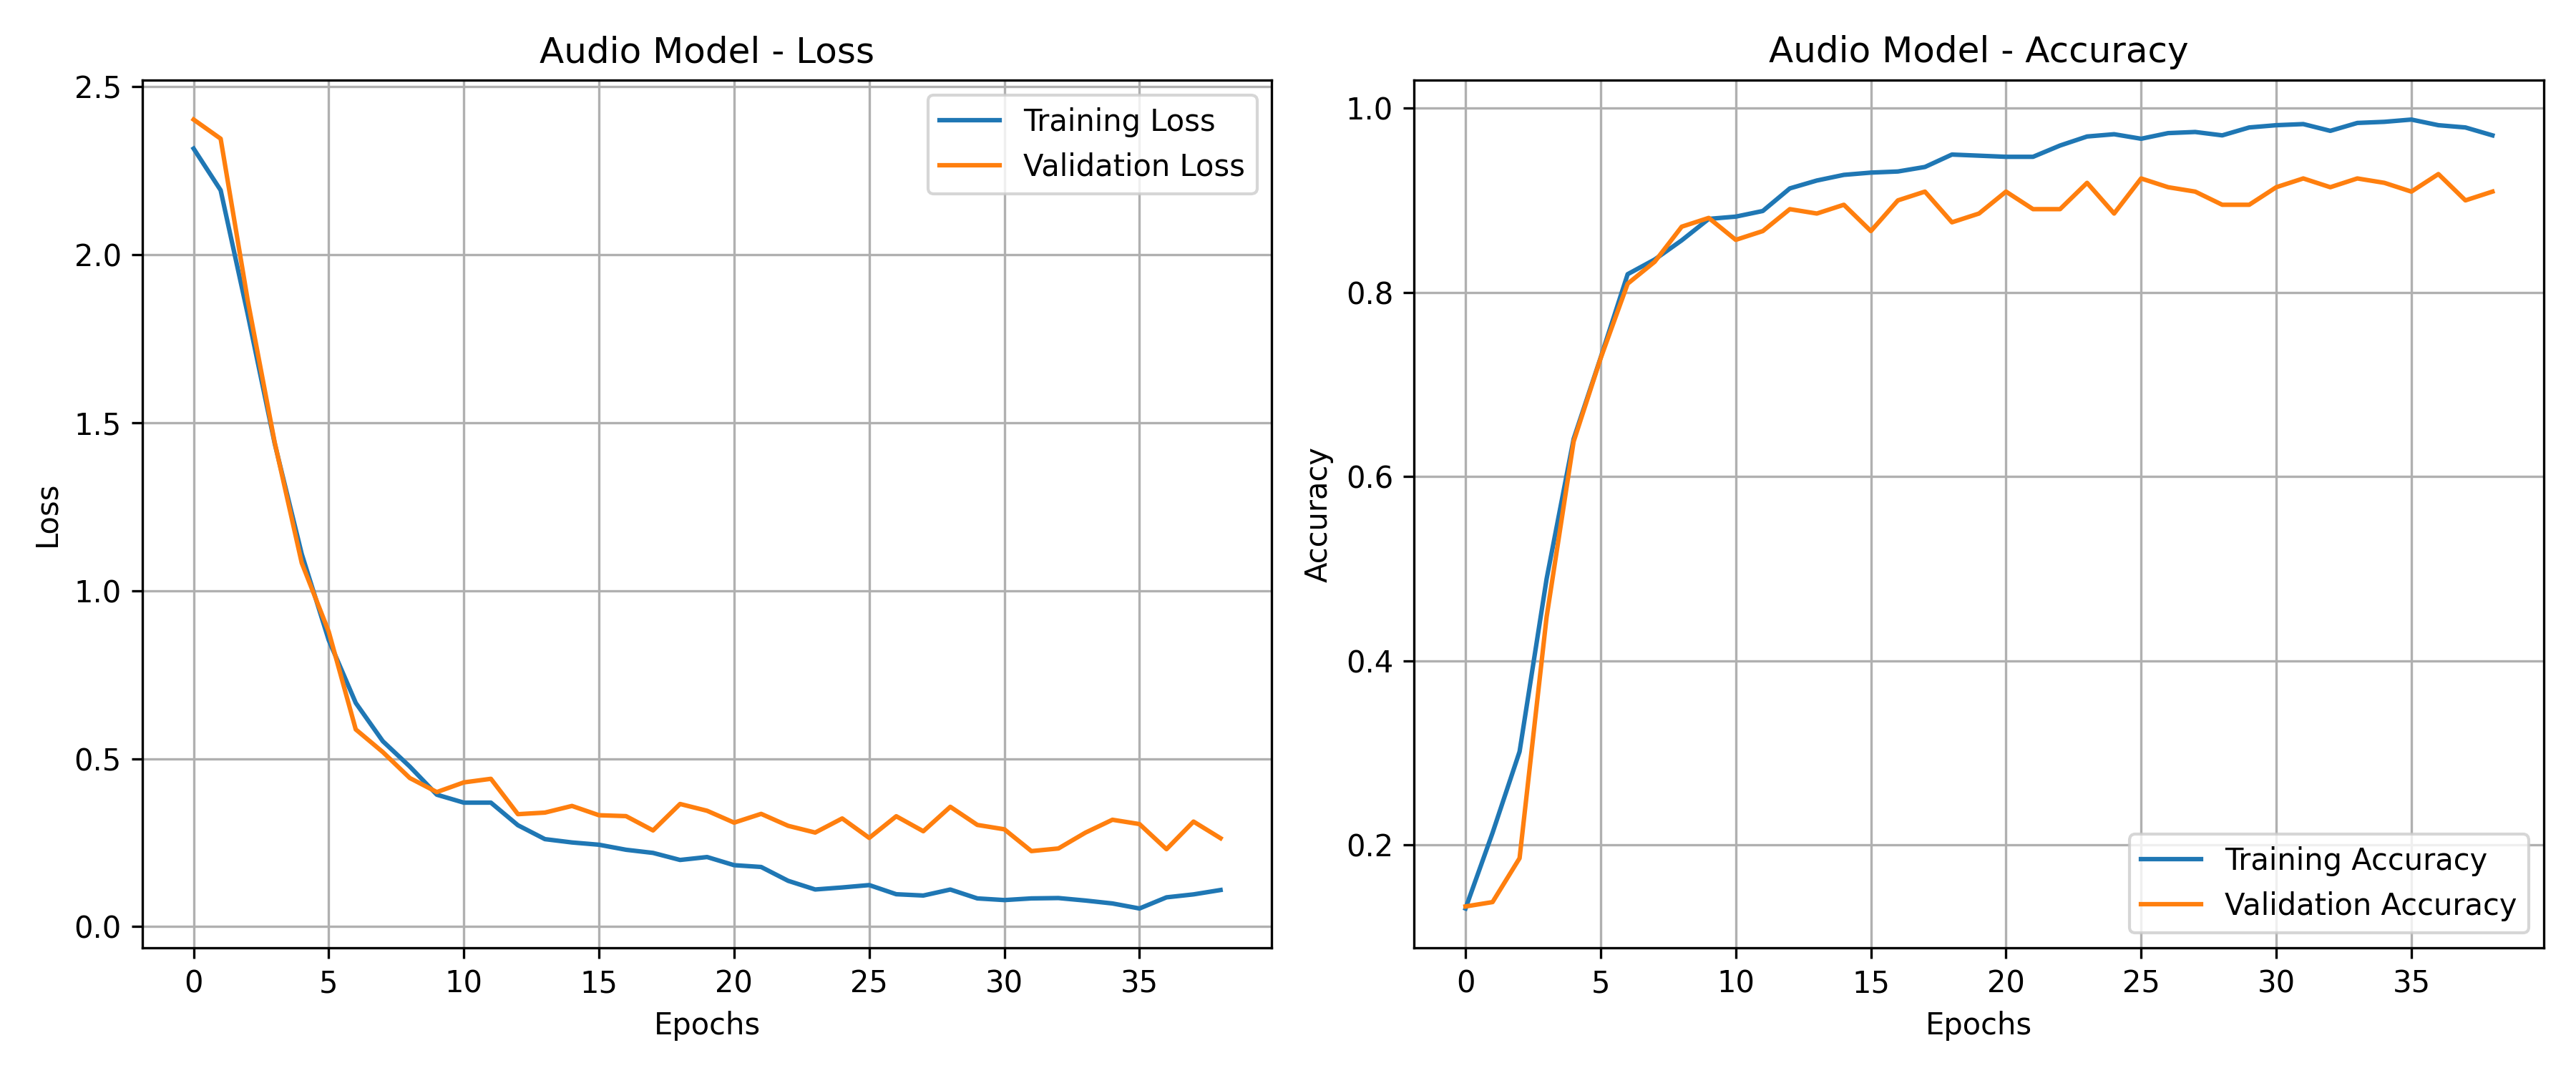
\includegraphics[width=\textwidth]{assets/audio_learning_curves.png}
  \caption{Learning curves of the Audio-Only LSTM model (accuracy and loss).}
  \label{fig:audio_curves}
\end{figure*}

\begin{figure*}[h]
  \centering
  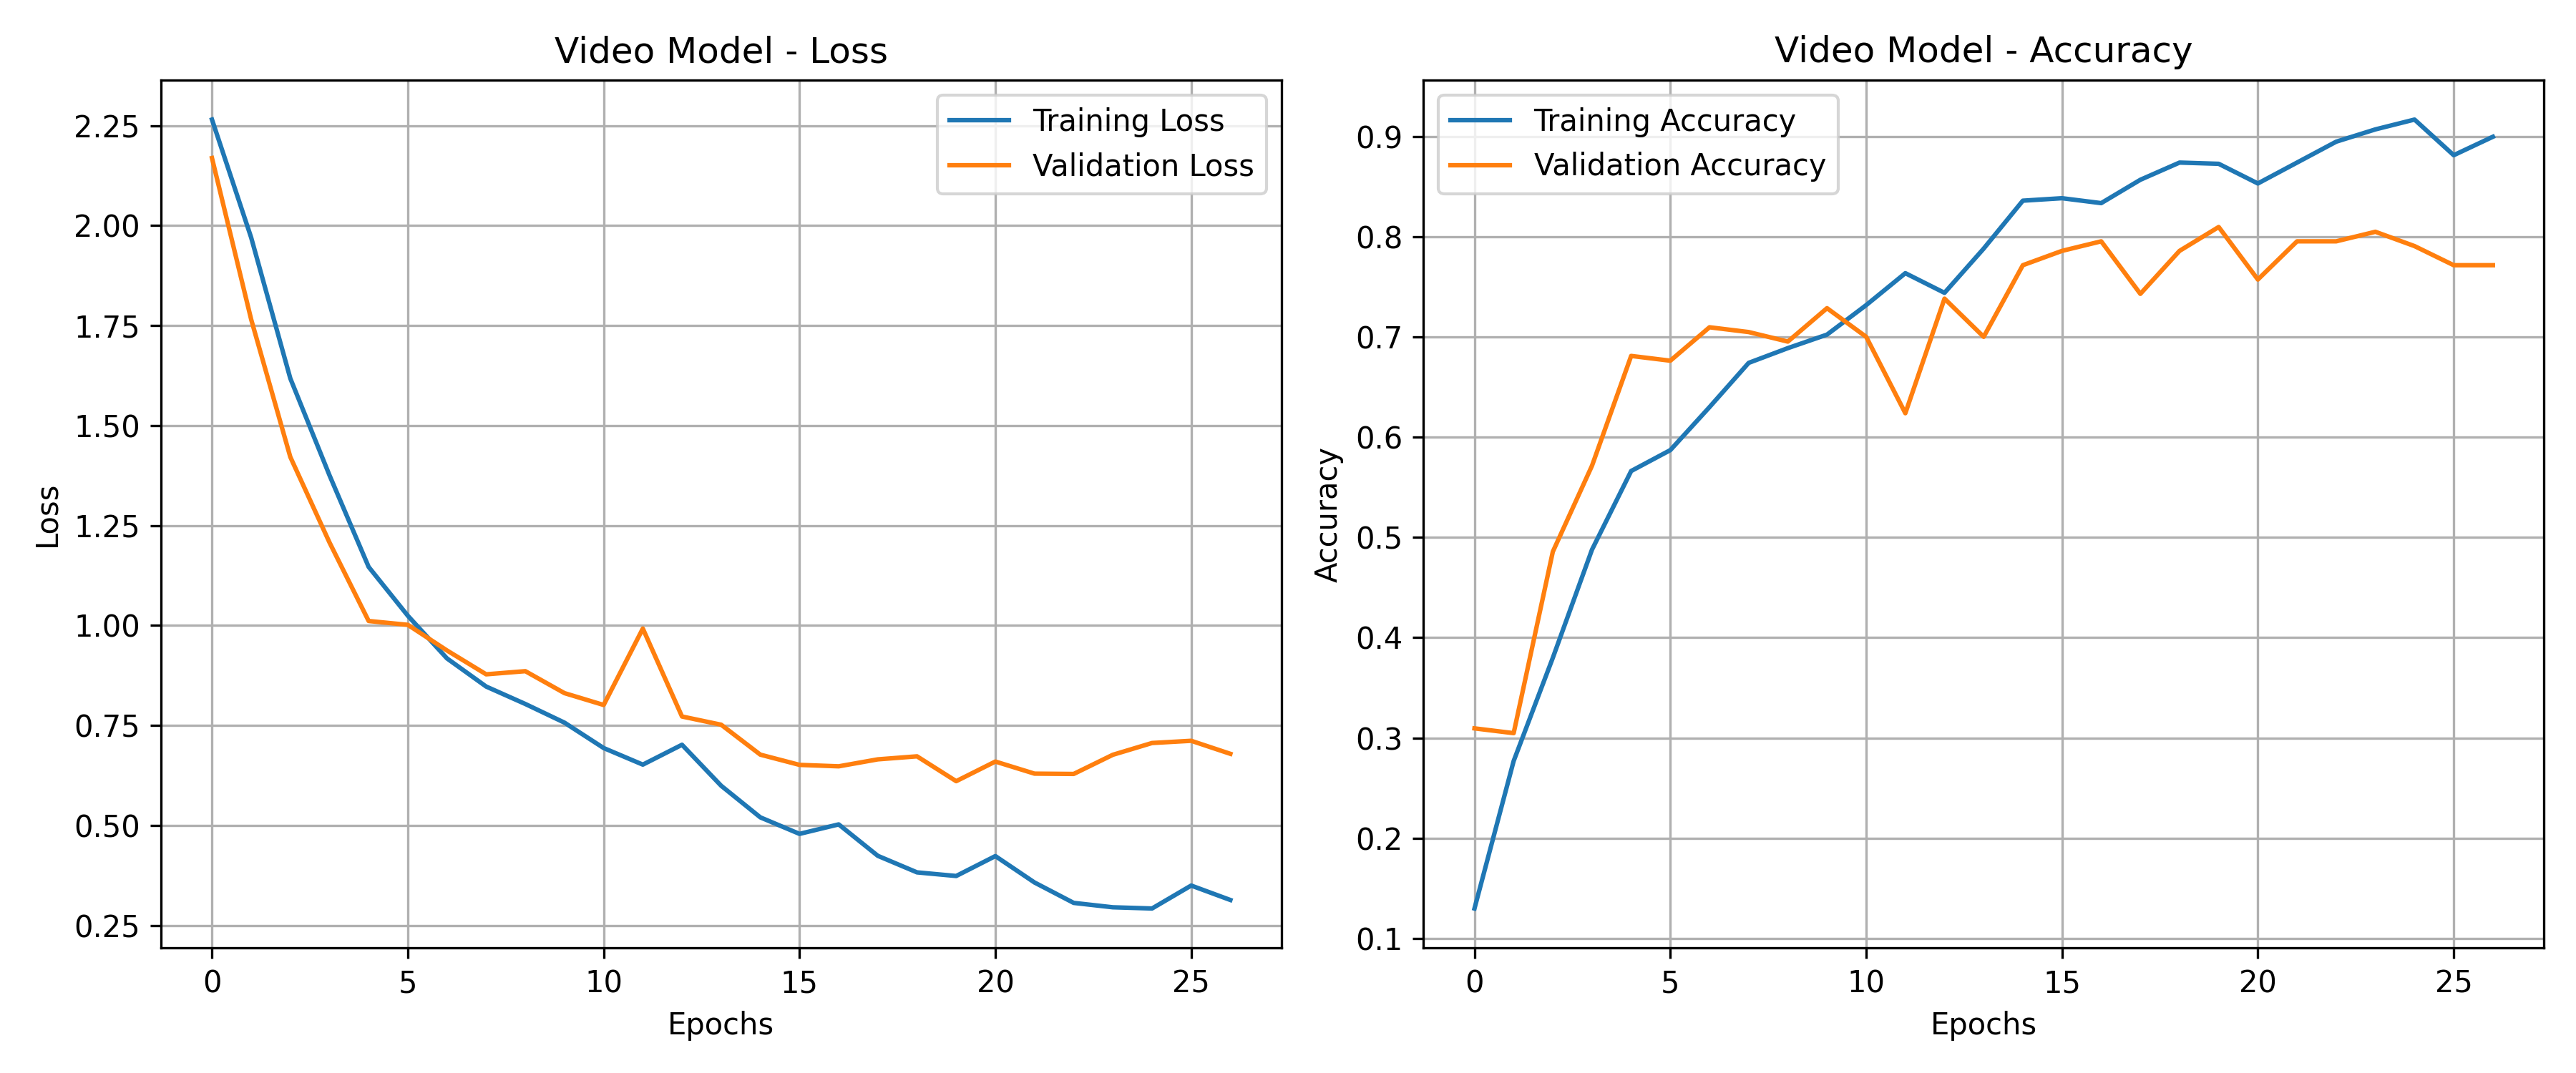
\includegraphics[width=\textwidth]{assets/video_learning_curves.png}
  \caption{Learning curves of the Video-Only BiLSTM model (accuracy and loss).}
  \label{fig:video_curves}
\end{figure*}

\begin{figure*}[h]
  \centering
  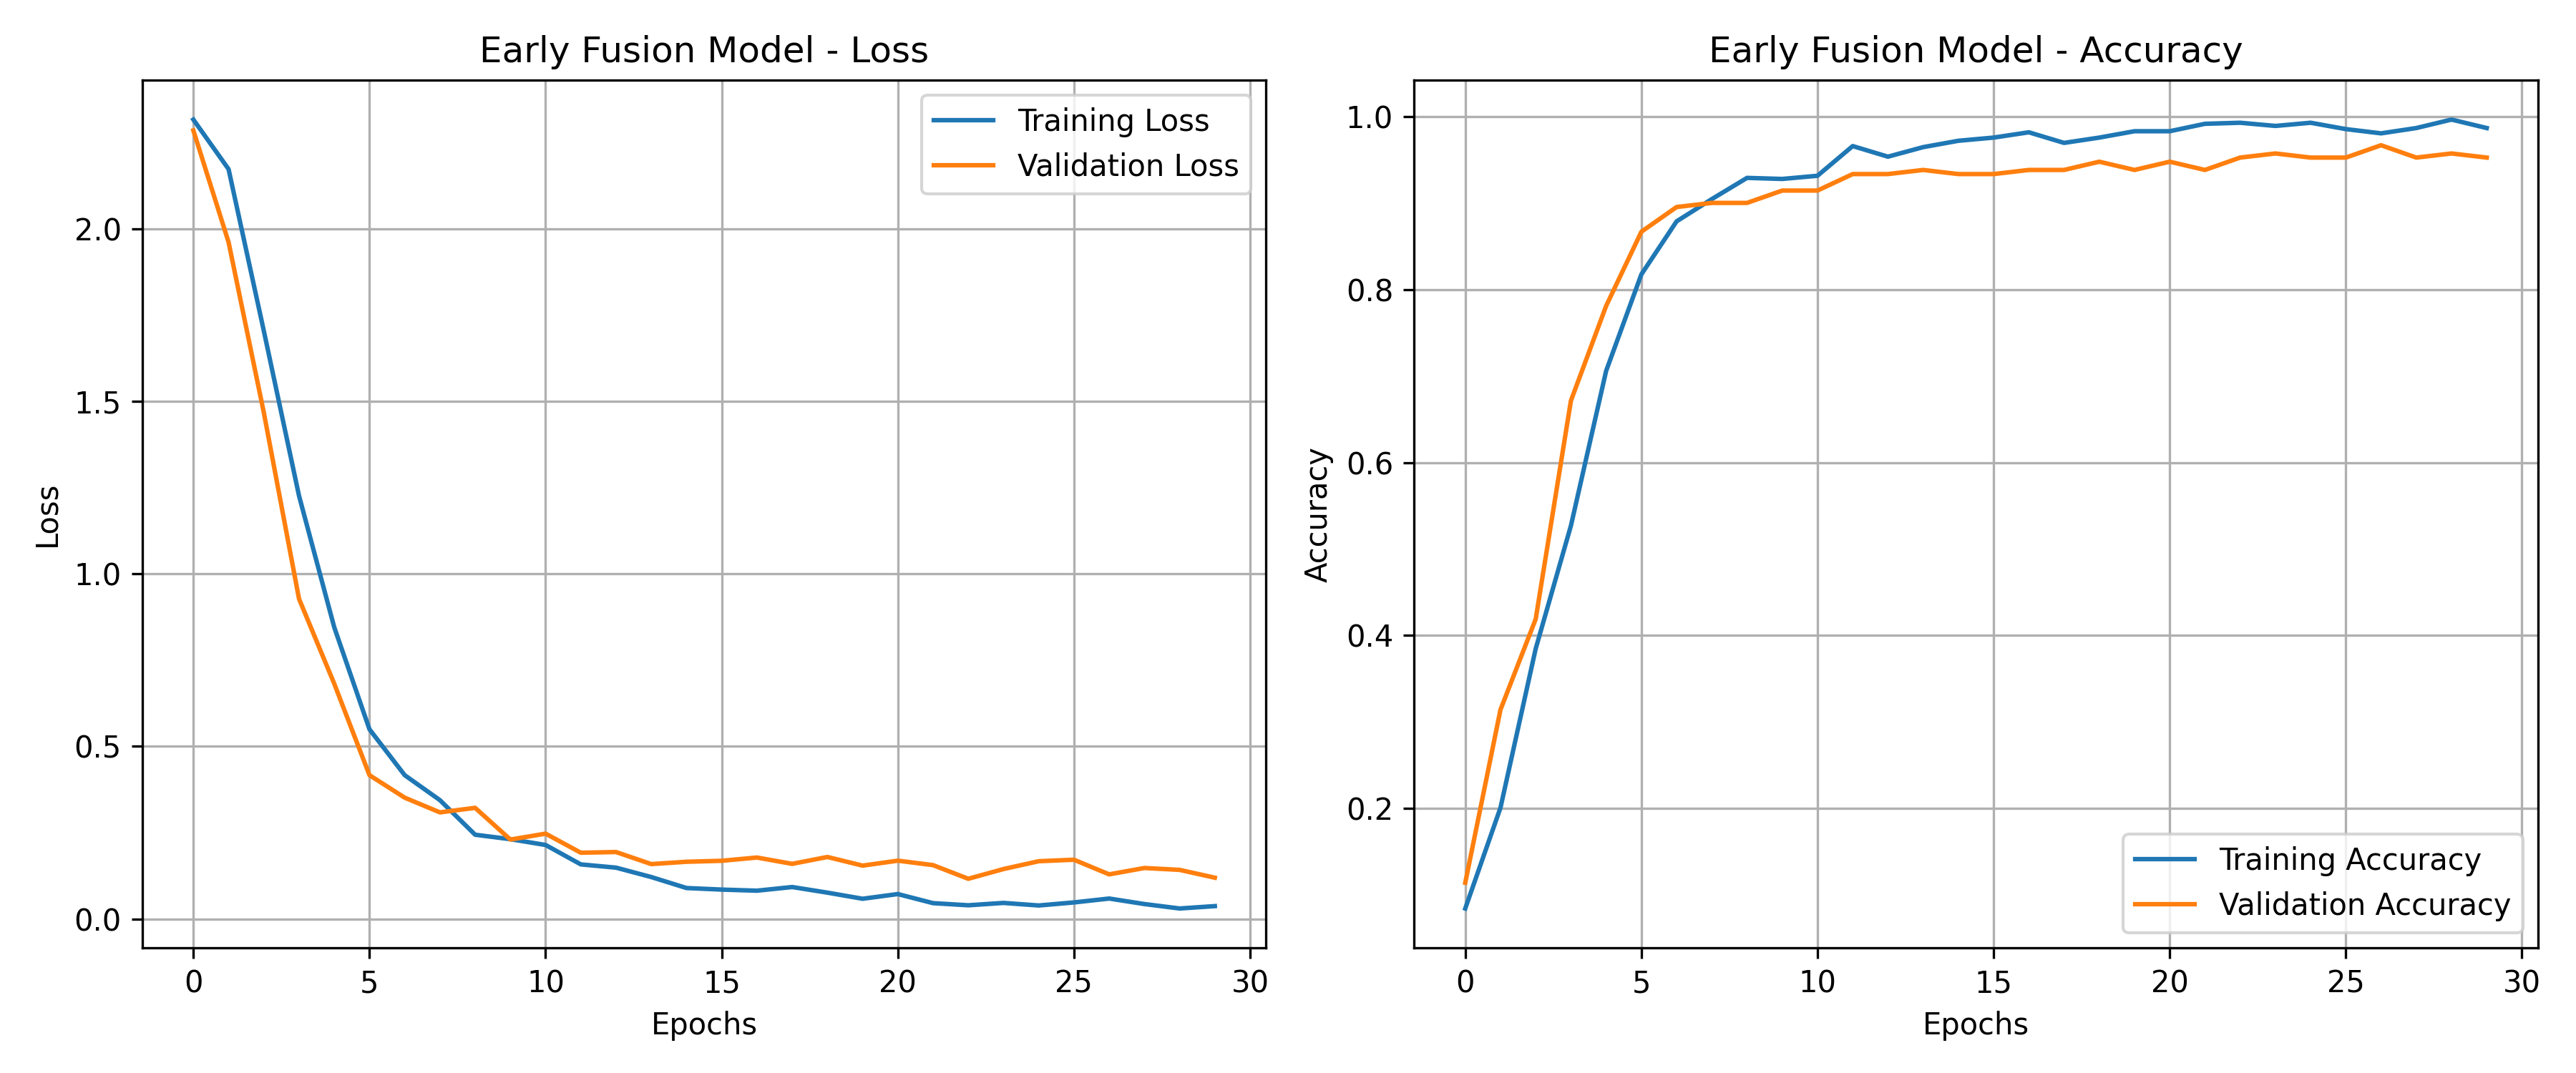
\includegraphics[width=\textwidth]{assets/fusion_learning_curves.png}
  \caption{Learning curves of the Early Fusion model (accuracy and loss).}
  \label{fig:fusion_curves}
\end{figure*}

The Audio-Only model converges in a relatively stable manner, with the validation accuracy closely tracking the training accuracy. The Video-Only model shows slower and slightly more unstable convergence, consistent with the greater difficulty of lip-reading using only geometric features. The fusion model shows the fastest convergence of the three, confirming that the availability of both modalities makes the classification task easier for the network.

\subsection{Confusion Matrices}

The confusion matrices in Figures~\ref{fig:audio_cm}, \ref{fig:video_cm}, and \ref{fig:fusion_cm} show the prediction distribution for each model across the full augmented Test set.

\begin{figure}[ht]
  \centering
  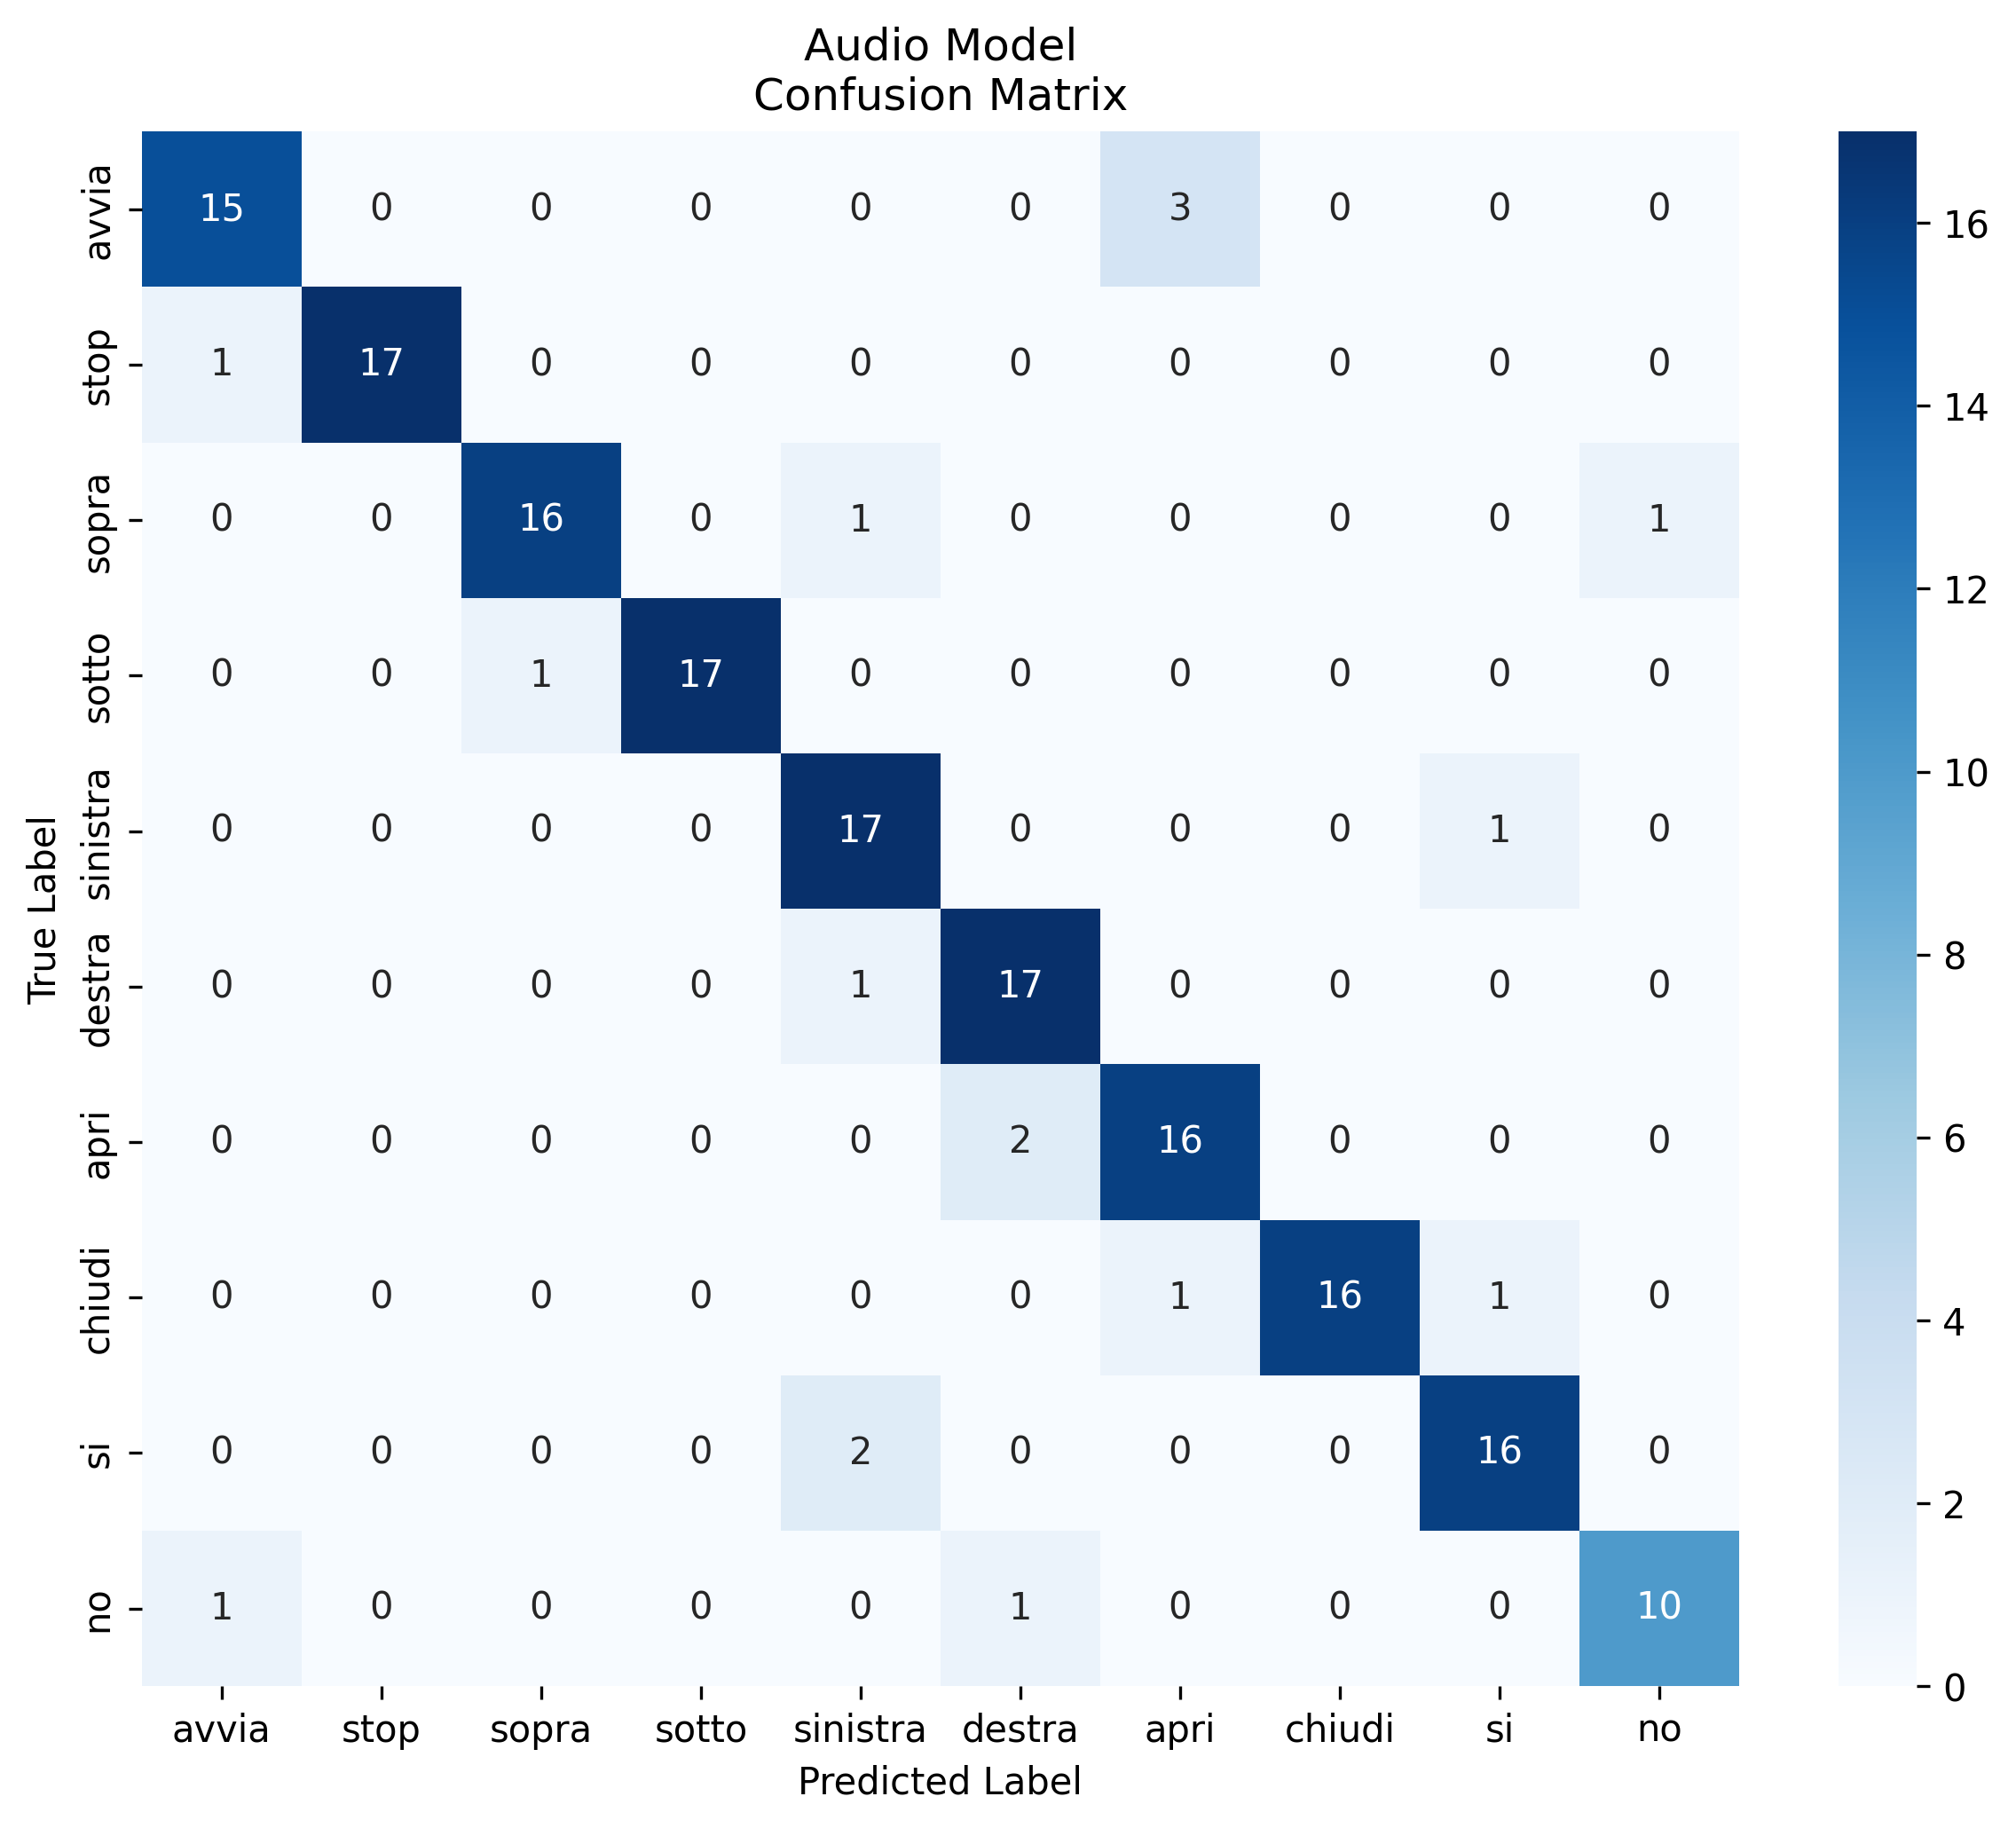
\includegraphics[width=\columnwidth]{assets/audio_confusion_matrix.png}
  \caption{Confusion matrix of the Audio-Only LSTM model.}
  \label{fig:audio_cm}
\end{figure}

\begin{figure}[ht]
  \centering
  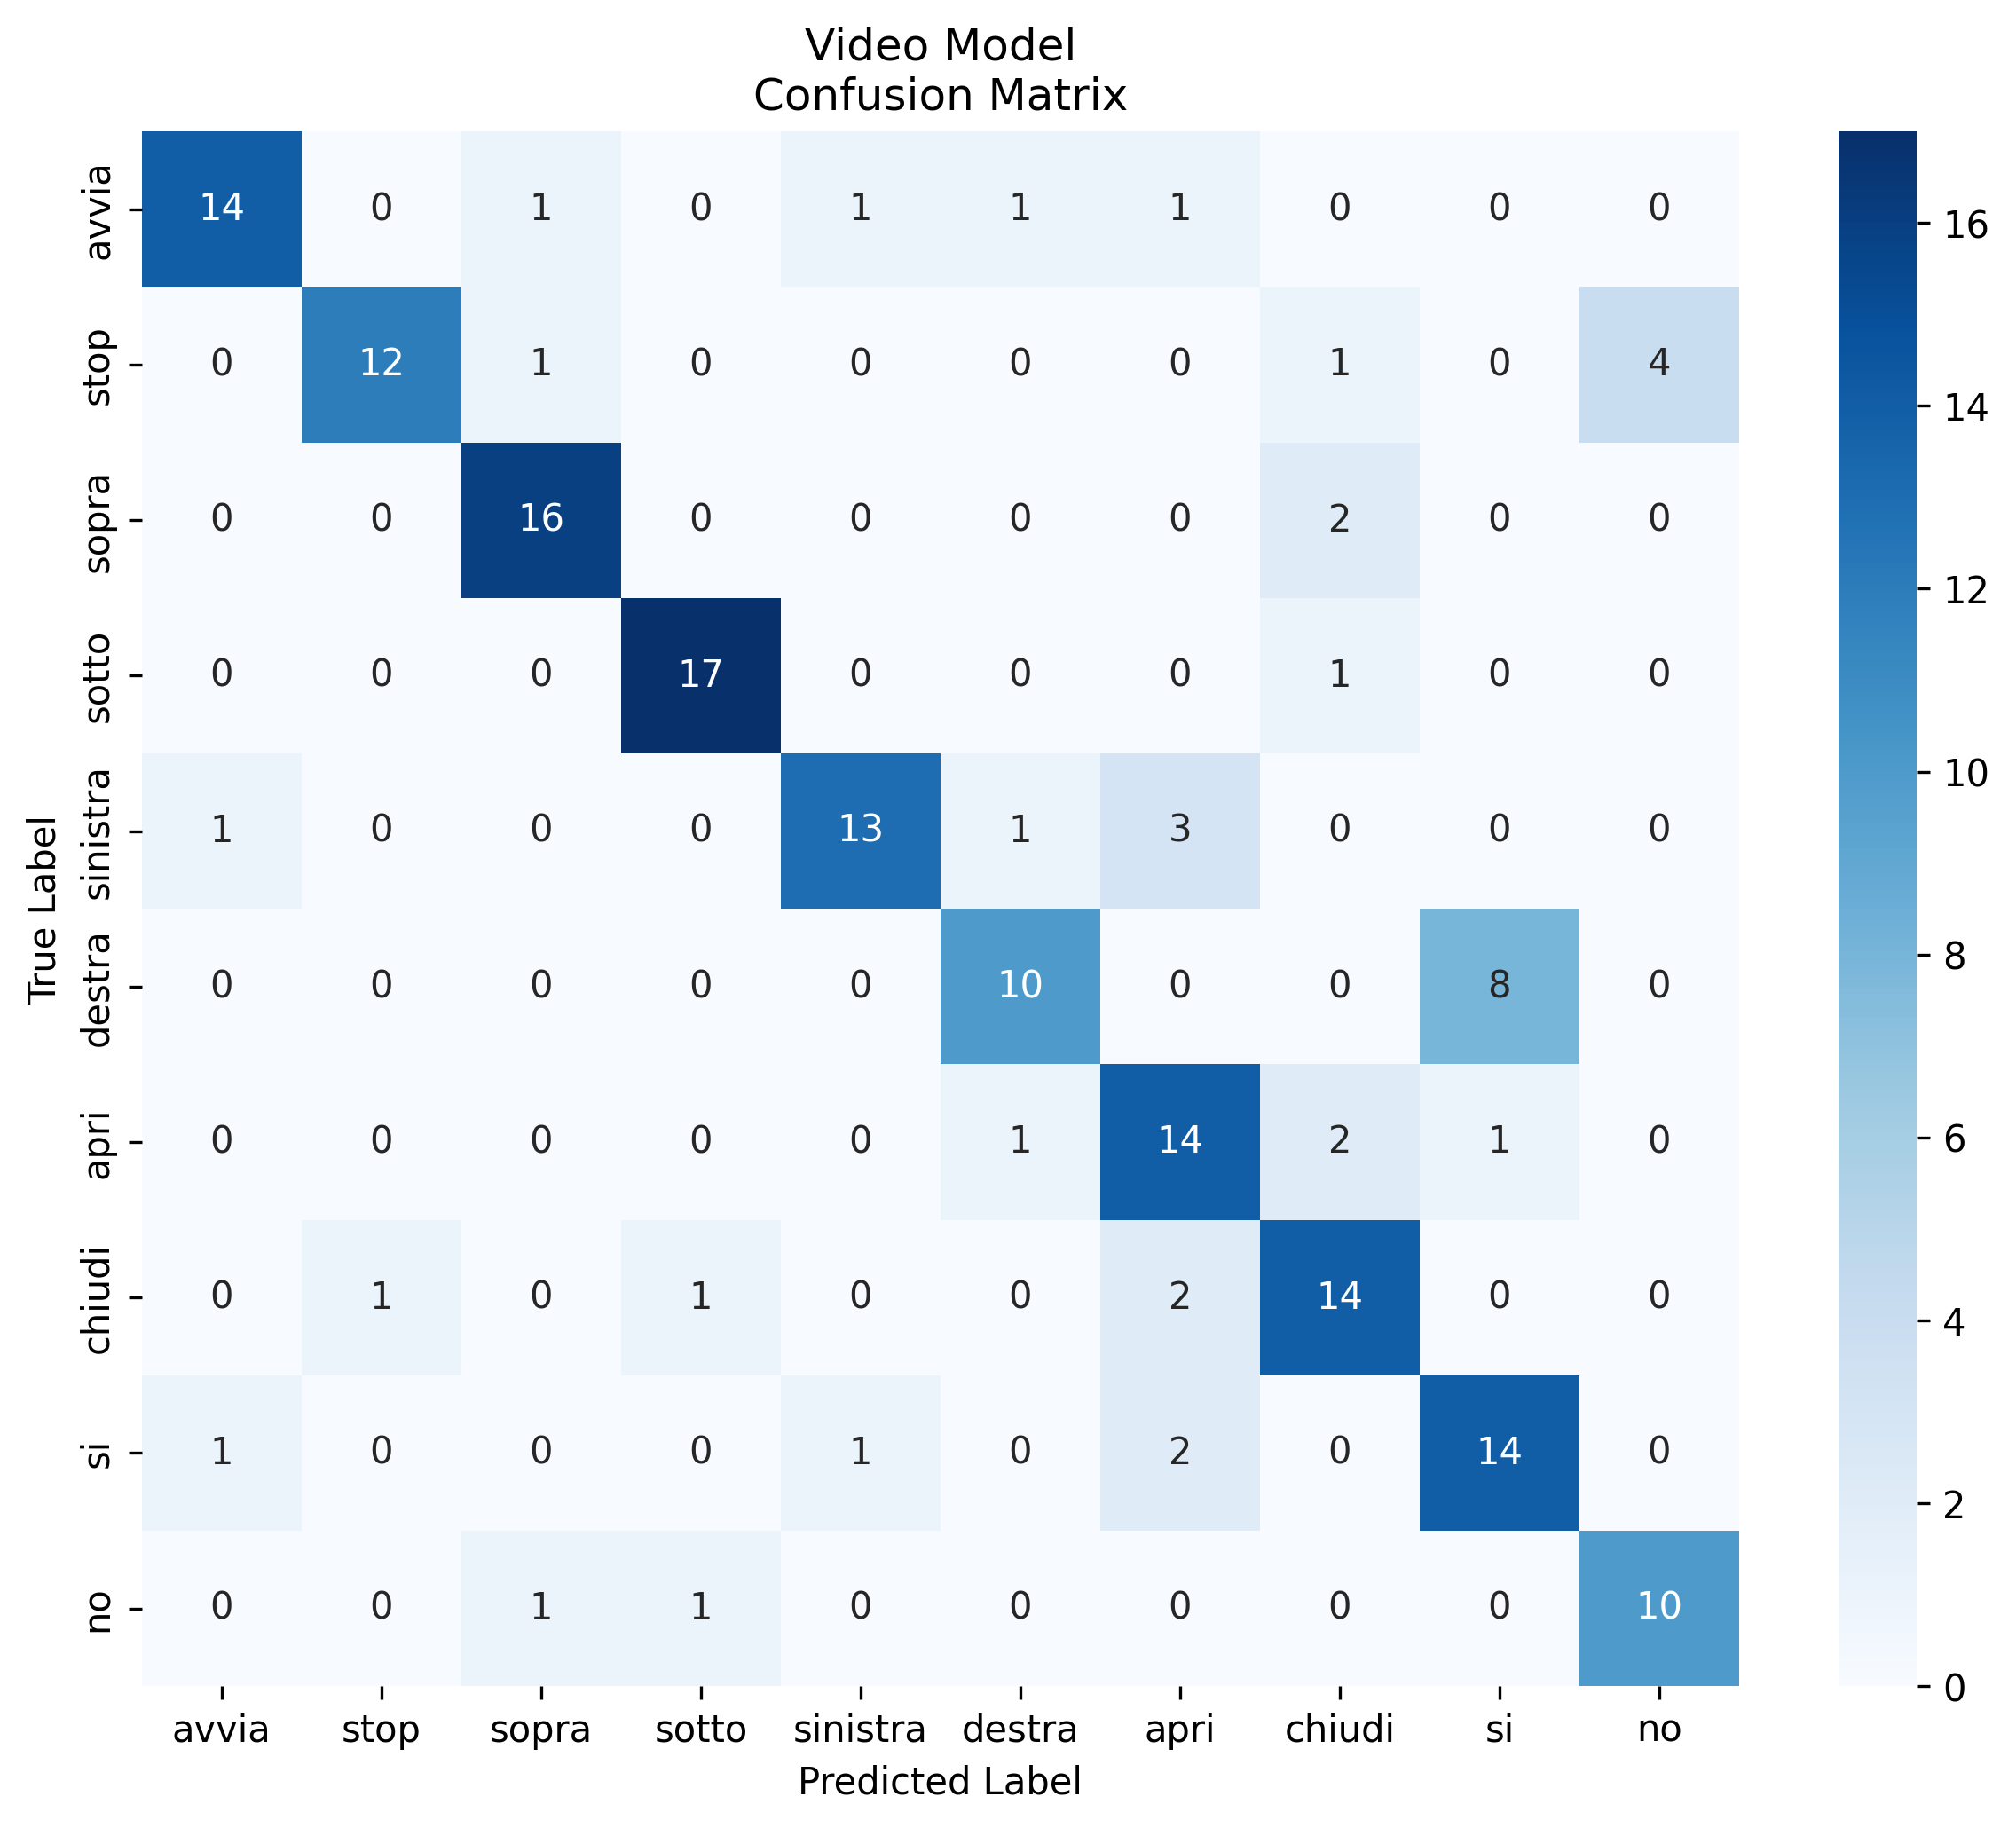
\includegraphics[width=\columnwidth]{assets/video_confusion_matrix.png}
  \caption{Confusion matrix of the Video-Only BiLSTM model.}
  \label{fig:video_cm}
\end{figure}

\begin{figure}[ht]
  \centering
  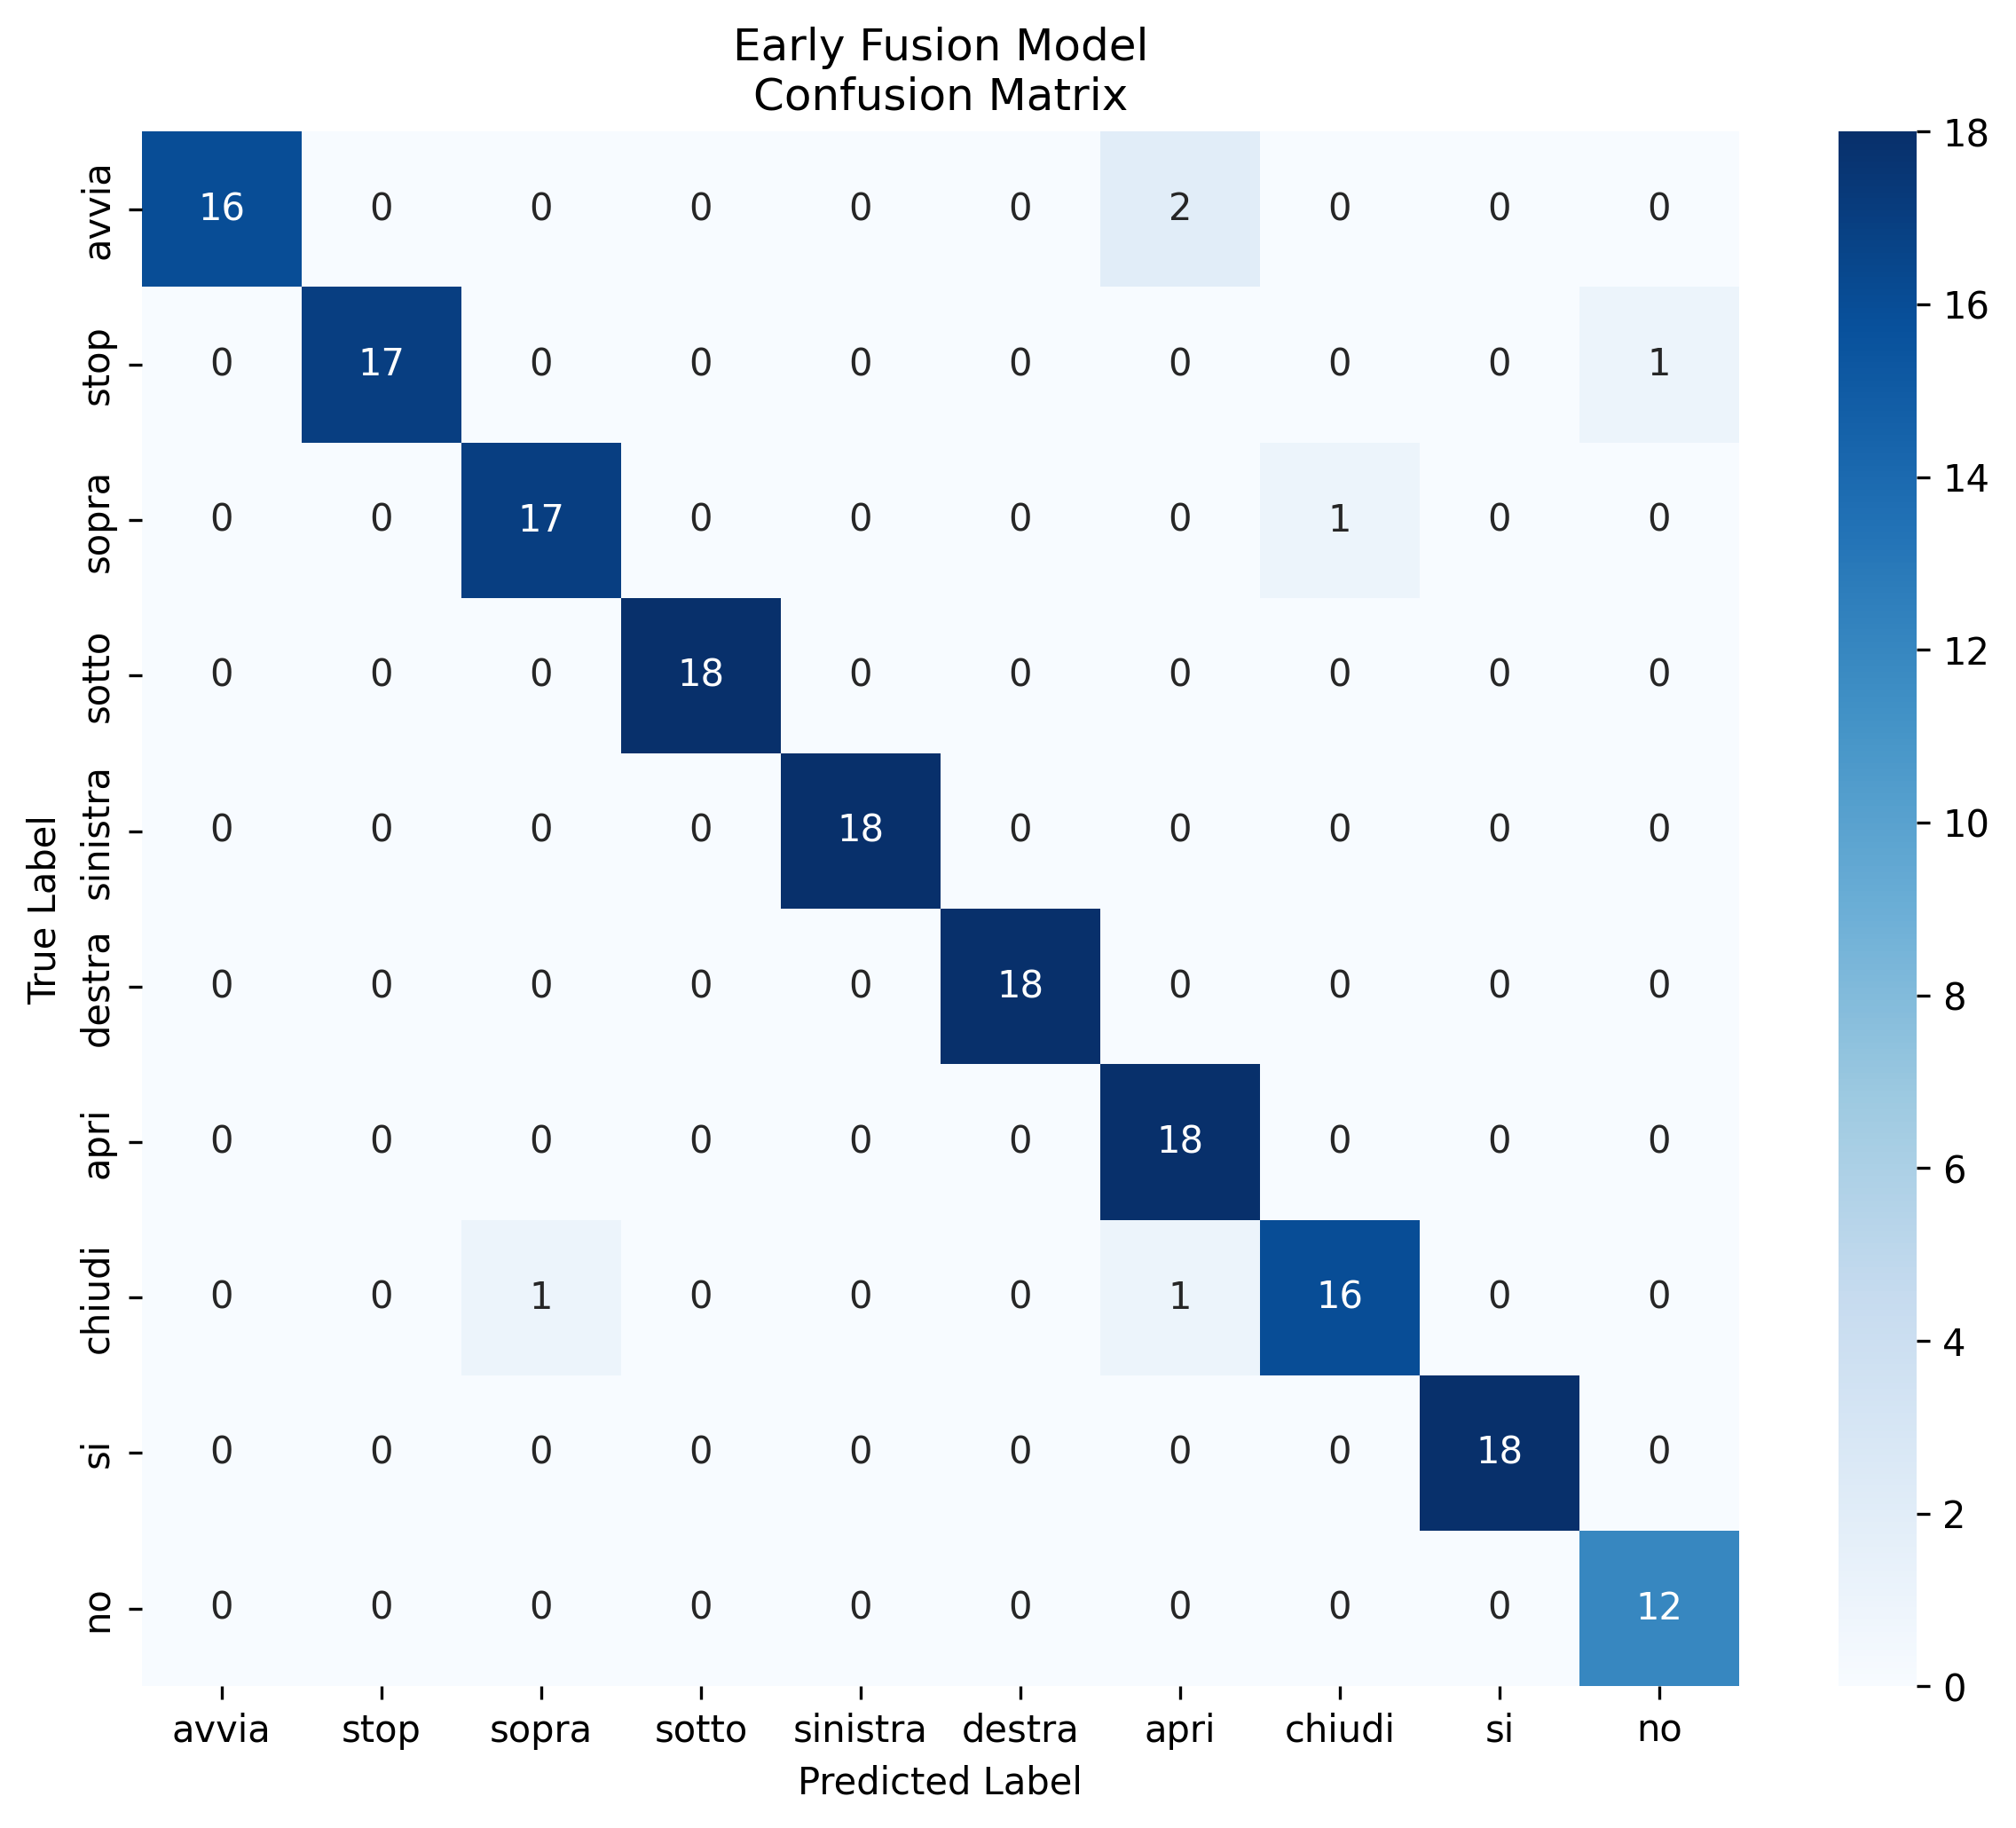
\includegraphics[width=\columnwidth]{assets/fusion_confusion_matrix.png}
  \caption{Confusion matrix of the Early Fusion model.}
  \label{fig:fusion_cm}
\end{figure}

The audio model's confusion matrix shows the largest errors in the Audio Heavy condition, where -15dB babble noise completely masks speech formants. The video model shows its main error cluster in the Video Light (Jitter) condition, where the kinematic derivatives $\Delta$ and $\Delta\Delta$ are destroyed by high-frequency perturbation. The fusion model has the cleanest diagonal, with residual errors primarily in the Audio Heavy condition.

\subsection{Unimodal Robustness and Orthogonality}

The empirical data clearly demonstrate the orthogonal independence of the two modalities. As expected, the Video-Only baseline is completely invariant to acoustic degradation, maintaining a stable accuracy of 96.55\% even in the \textit{Audio Heavy} (-15dB) condition. Conversely, the acoustic model drops to 44.83\% under the same noise, as babble noise completely masks the speech formants.

Similarly, the modalities show opposite vulnerabilities. The Video-Only model suffers a catastrophic failure in the \textit{Video Light} (Jitter) condition, dropping to 41.38\%. The rapid frame-by-frame perturbation destroys the kinematic derivatives $\Delta$ and $\Delta\Delta$, making lip-reading impossible. Under this condition, the Audio-Only model remains unaffected (100.00\%). Notably, the static \textit{Video Heavy} (Tilt) condition did not significantly impair the visual model (96.55\%), demonstrating that the MediaPipe topology and normalization layers are rotation-invariant, while they are highly sensitive to high-frequency jitter.

\subsection{Multimodal Synergy and Dynamic Gating}

The Early Fusion model achieved an overall accuracy of 96.55\%, clearly outperforming both unimodal baselines (90.23\% and 77.01\%). The fusion network demonstrated ``soft-gating'' capabilities --- the ability to dynamically weight the most reliable modality:
\begin{itemize}
  \item \textbf{Audio recovery:} In the \textit{Audio Heavy} condition, where the acoustic model failed (44.83\%), the visual features acted as an anchor, bringing fusion performance to 86.21\% (an absolute recovery of +41.38 percentage points).
  \item \textbf{Video recovery:} In the \textit{Video Light} condition, where the visual model failed (41.38\%), the network ignored the corrupted kinematics and relied entirely on the clean audio, achieving a perfect accuracy of 100.00\%.
\end{itemize}

\subsection{Observations on Modality Interference}

Although the fusion model consistently matches or exceeds the best available unimodal baseline, the \textit{A+V Light} condition highlights a fundamental challenge in multimodal learning. When both modalities are degraded simultaneously (babble noise + jitter), the network receives conflicting, low-confidence signals from both branches. In this experiment, the fusion model achieved 96.55\%, matching the Audio-Only baseline and effectively preventing negative transfer, but without finding synergistic improvements when both input channels are compromised.

This result suggests that simple feature concatenation (Early Fusion) has limited capacity to handle scenarios where both modalities are degraded: the network learns to ignore the worse modality, but lacks an explicit mechanism to dynamically modulate attention over individual frames or features.

\section{Conclusions and Future Work}

This report presented an AVSR system designed to maintain high classification accuracy in degraded acoustic and visual environments. By engineering kinematic spatial derivatives ($\Delta$ and $\Delta\Delta$) from facial landmarks, the visual modality was provided with the dynamic context needed to accurately decode lip movements.

A central aspect of the work was the systematic identification and resolution of two common experimental biases: Data Leakage and Padding Bias. By adopting a Stratified Group K-Fold strategy and the Continuous Noise Canvas technique, it was ensured that the network's predictive power derived from genuine cross-modal representations rather than artificial heuristics or duration-based shortcuts.

Empirical evaluations across a 6-condition Ablation Matrix demonstrated the superiority of the Early Fusion architecture. The multimodal system achieved an overall accuracy of 96.55\%, effectively using the visual modality to recover the acoustic branch under catastrophic -15dB Babble Noise (+41.38 percentage points recovery), while simultaneously ignoring degraded visual kinematics during high-frequency spatial jitter.

Despite these positive results, the phenomenon of modality interference remains an open challenge. When both modalities are degraded with conflicting noise profiles, simple feature concatenation (Early Fusion) struggles to dynamically route the network's attention.

\subsection{Residual Error Analysis}

A qualitative analysis of the fusion model's residual errors reveals interesting patterns. Commands sharing similar phonetic characteristics (e.g., \textit{sopra} and \textit{stop}, which share the initial /s/ sound) account for the majority of misclassifications. Similarly, at the visual level, commands with similar lip movements (e.g., \textit{apri} and \textit{avvia}, which both begin with the bilabial movement /a/) are harder to distinguish for the visual branch.

The fusion model manages to resolve some of these ambiguities because phonetically similar pairs are not necessarily visemically similar, and vice versa. However, when a pair of commands shares both phonetic and visemic similarities, fusion does not offer advantages over the unimodal baselines.

\subsection{Dataset Considerations}

The collected dataset, while sufficient for this exploratory study, presents some structural limitations. First, the data comes from a single speaker, which limits inter-subject variability. Second, recordings were made in a controlled environment with uniform lighting and a fixed background, whereas real-world conditions can vary significantly.

Despite these limitations, the experimental framework built --- with its augmentation pipeline and anti-bias strategies --- is designed to scale to larger and more diverse datasets without substantial architectural modifications.

\textbf{Future work:} To address these limitations, future iterations of the system could explore \textit{Cross-Modal Attention} mechanisms and Transformer-based architectures, which allow the network to assign dynamic attention weights to specific frames of each modality. Expanding the dataset to a continuous-speech vocabulary with diverse speaker profiles would further test the system's zero-shot generalization capabilities. Finally, optimizing the inference pipeline for edge-device deployment --- via quantization techniques --- would translate this robust AVSR architecture into real-time assistive technologies.

\bibliographystyle{ACM-Reference-Format}
\bibliography{main}

\end{document}
